\documentclass{article}
\usepackage{brian}
\usepackage{hyperref}

\title{Onset entropy and rhythm analysis}
\author{Brian McFee}

\begin{document}
\maketitle

\section{Beat tracking and information gain}

Let $b^r, b^p \in \{0,1\}^T$ denote a reference ($b^r$) and predicted ($b^p$) collection of beats
for a song: 
    \[
        b_t \defeq \ind{\text{there is a beat at time } t}.
    \]

Now, define the (unnormalized) cross-correlation as:
\[
\left[\rho(b^r, b^p)\right]_\delta \defeq \E_t \left[b^r_t b^p_{t+\delta} \right]
\]
where $\delta$ is a discrete lag value lying within some bounded interval.
We may then normalize to form a distribution:
\[
\rho \mapsto \frac{\rho}{\sum_\delta \rho_\delta}.
\]

(Some guys) define the negentropy of $\rho$ as a means of measuring the accuracy of the prediction $b^p$ with 
respect to the reference beats $b^r$:

\[
H(\rho) \defeq - \sum_\delta \rho_\delta \log \rho_\delta.
\]

The key idea here is that even if predicted beats don't directly coincide with the reference, if they're
consistently off, then $\rho$ will be strongly peaked, and thus have low negentropy.

\section{Onset correlation}
We can generalize the above idea by relaxing to continuous-valued vectors: $o^p \in [0,1]^t$ where 
\[
    o_t \defeq \text{normalized onset strength at time } t.
\]

The above negentropy calculation can then be performed against a reference beat pulse train $b^r$, or an
alternative onset profile $o^r$ (\eg, one derived from a specific frequency sub-band).  
In the latter case, the negentropy score may be used to evaluate the synchronicity (accounting for lag) between
$o^r$ and $o^p$.

In particular, the negentropy of the autocorrelation $\rho(o^p, o^p)$ can be used to estimate
the stability of a particular onset profile.


\section{Beat tracking revisited}

This idea can be useful in determining where in the frequency range the beat is being stated (if at all): sometimes the beat is indicated by bass (low-end), and other times, the beat is driven
by cymbals (broad-band, but easily detected at the high-end).  See \autoref{fig:oe}. 

\begin{figure}
\centering%
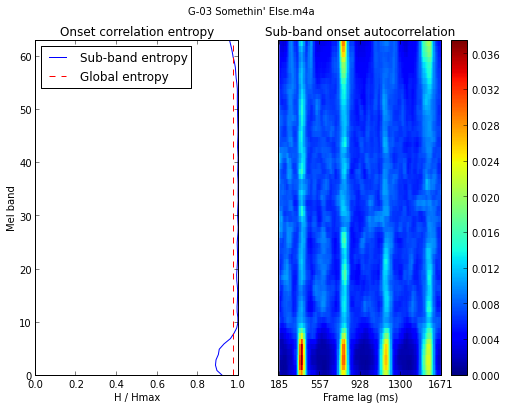
\includegraphics[width=0.75\textwidth]{oe-bass}\\
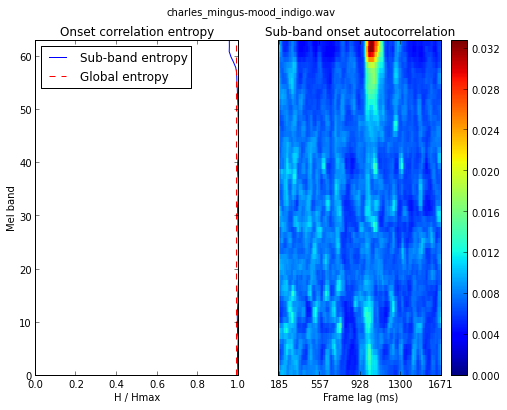
\includegraphics[width=0.75\textwidth]{oe-treble}%
\caption{Sub-band onset auto-correlation and entropy for two songs.  ``Global onset'' refers to the onset profile derived from all frequency bands.\label{fig:oe}}
\end{figure}

Rather than taking a uniform weighting of spectral difference across frequency bands (as is currently done in the DPWE tracker),
we could use per-band entropy estimates to weight individual onset profiles:
\[
o^* \defeq \sum_f \frac{H(\rho(o^f, o^f))}{\sum_g H(\rho(o^g, o^g))} o^f.
\]

\section{Dynamic tracking}
Rather than a single, temporally-global weighting, it may make more sense to use sub-band entropy estimates which are calculated only locally (\eg, in a window of $\pm$60s).  This should allow
the tracker to adapt to different instruments stating the beat at different times within a song.

\end{document}
